\documentclass[12pt, titlepage]{article}

\usepackage{fullpage}
\usepackage[round]{natbib}
\usepackage{multirow}
\usepackage{booktabs}
\usepackage{tabularx}
\usepackage{graphicx}
\usepackage{float}
\usepackage{hyperref}
\hypersetup{
    colorlinks,
    citecolor=black,
    filecolor=black,
    linkcolor=red,
    urlcolor=blue
}
\usepackage[round]{natbib}

\newcounter{acnum}
\newcommand{\actheacnum}{AC\theacnum}
\newcommand{\acref}[1]{AC\ref{#1}}

\newcounter{ucnum}
\newcommand{\uctheucnum}{UC\theucnum}
\newcommand{\uref}[1]{UC\ref{#1}}

\newcounter{mnum}
\newcommand{\mthemnum}{M\themnum}
\newcommand{\mref}[1]{M\ref{#1}}

\title{SE 3XA3: Software Requirements Specification\\Tetrileet}

\author{Team 15, AAA Solutions
		\\ Student 1 Abdallah Taha, tahaa8
		\\ Student 2 Andrew Carvalino, carvalia
		\\ Student 3 Ali Tabar, sahraeia
}

\date{\today}

\begin{document}

\maketitle

\pagenumbering{roman}
\tableofcontents
\listoftables
\listoffigures
\newpage
\begin{table}[h!]
\caption{\bf Revision History}
\begin{tabularx}{\textwidth}{p{3cm}p{2cm}X}
\toprule {\bf Date} & {\bf Version} & {\bf Notes}\\
\midrule
March 16 2021 & 1.0 & Added sections 1, 2, 3, 5\\
March 17 2021 & 1.1 & Added sections 4, 6, 7\\
\textcolor{red}{April 12 2021} & \textcolor{red}{1.2} & \textcolor{red}{Added Anticipated changes AC5,AC6,AC7 and updated the traceability accordingly. Changed the Grid module to Behaviour-Hiding Module. Changed the secret of the Start Game Module. All changes were done in red.}\\
\bottomrule
\end{tabularx}
\end{table}

\newpage

\pagenumbering{arabic}

\section{Introduction}





Tetrileet is a redevelopment of LoveDaisy's Tetris found on GitHub, which is itself an adaptation to the classic video game known as \textit{Tetris}. The original project was made in Python, but our remake is in JavaScript. Our main goal with this project is to improve upon the preexisting implementation, by adding or adjusting program aspects - all of these changes have been touched upon and explained in the Software Requirements Specification (SRS). The intentions behind these changes are to create a more accessible, user-friendly, and customized experience, enticing longer play times from users.
\\One of the most commonplace and widely accepted methods to software development is modular design. This entails the division of a software system into multiple different components called modules. We selected this method to ensure better manageability and maintainability for our project, while following the principle of information hiding. This will support maintainability in the future, especially if any changes are to be made to the software.\\
From this MG, we created the Module Interface Specification (MIS) to showcase the details regarding the implementation of every module.
\\The Module Guide's (MG) main purpose is to describe the design of the software from a modular perspective to readers. Readers can include:

\begin{itemize}
\item New members of AAA solutions who are joining the Tetrileet development team:
\\The module guide is a valuable resource for a member of the development team to 
  conceptually grasp the design of the overall project, and also to find information for specific modules of interest.
\item Current maintainers of the project: Before making changes to the system, a maintainer should have a concise understanding of the software system's hierarchy. The module guide can help ensure this. Additionally, if changes are made to the system, other maintainers can become aware of this through the MG, as the maintainer who made the changes should update the module guide to reflect them.
\item Current designers of the project: Designers can use the MG to ensure consistency, feasibility and flexibility in the system - modules must be consistent with one another to work, the deconstruction of the entire system should be convenient and intuitive, and the design as a whole should be flexible - allowing designers to tweak various aspects without difficulty.  
\end{itemize}

The rest of the document is organized as follows:


\begin{itemize}
\item Section 2: a list of changes in the software requirements, both anticipated and unlikely
\item Section 3: an overview of the module decomposition created from the likely changes
\item Section 4: the connections between the software requirements and modules of the design
\item Section 5: detailed descriptions of modules
\item Section 6: traceability matrices which check completeness of the design against SRS requirements and show the relation between anticipated changes and modules
\item Section 7: a diagram showcasing the use relations between modules
\end{itemize}




\section{Anticipated and Unlikely Changes} \label{SecChange}

This section lists possible changes to the system that may or may not be implemented at a later time. Changes which are anticipated to be implemented are listed in Section \ref{SecAchange}, and
unlikely changes to the project are listed in Section \ref{SecUchange}.

\subsection{Anticipated Changes} \label{SecAchange}

\begin{description}
\item[\refstepcounter{acnum} \actheacnum \label{acBrowser}:] 
The web browser the player uses to run the application and how the scripting and styling modules account for those differences.
\item[\refstepcounter{acnum} \actheacnum \label{acWindow}:] 
The size of the browser window the player uses and how the game fits inside it.
\item[\refstepcounter{acnum} \actheacnum \label{acModules}:] 
The internal implementation of existing modules.
\item[\refstepcounter{acnum} \actheacnum \label{acUI}:] 
The User Interface of the game and how objects are displayed.
\item[\refstepcounter{acnum} \actheacnum \label{acGF}:] 
\textcolor{red}{Added different shapes to the game.}
\item[\refstepcounter{acnum} \actheacnum \label{acModules}:] 
\textcolor{red}{Some Modules may be combined if found to be more efficient in development.}
\item[\refstepcounter{acnum} \actheacnum \label{acTesting}:] 
\textcolor{red}{Testing methods may be changed if new ones are found that are more efficient.}


\end{description}

\subsection{Unlikely Changes} \label{SecUchange}

\begin{description}
\item[\refstepcounter{ucnum} \uctheucnum \label{ucInput}:] 
Alternate input devices, such as a video game console controller or a touch pad.
\item[\refstepcounter{ucnum} \uctheucnum \label{ucAudio}:] 
Adding sound effects to the game, such as menu music or block placement sounds.
\item[\refstepcounter{ucnum} \uctheucnum \label{ucDevice}:] 
The user running the game on an alternate device, such as a phone or through a web browser on a video game console.
\item[\refstepcounter{ucnum} \uctheucnum \label{ucPlayers}:] 
Implementing a multiplayer feature in the game.
\end{description}

\newpage
\section{Module Hierarchy} \label{SecMH}

This section lists all existing modules and showcases the module design. Modules are displayed in their hierarchy in Table \ref{TblMH}.

\begin{description}
\item [\refstepcounter{mnum} \mthemnum \label{mHH}:] Game Window
\item [\refstepcounter{mnum} \mthemnum \label{mHH}:] Start Game
\item [\refstepcounter{mnum} \mthemnum \label{mHH}:] Pause Game
\item [\refstepcounter{mnum} \mthemnum \label{mHH}:] End Game
\item [\refstepcounter{mnum} \mthemnum \label{mHH}:] Grid
\item [\refstepcounter{mnum} \mthemnum \label{mHH}:] Game Controller
\item [\refstepcounter{mnum} \mthemnum \label{mHH}:] Shape
\item [\refstepcounter{mnum} \mthemnum \label{mHH}:] BlockStack
\item [\refstepcounter{mnum} \mthemnum \label{mHH}:] RowCheck
\item [\refstepcounter{mnum} \mthemnum \label{mHH}:] BlockFall

\end{description}


\begin{table}[h!]
\centering
\begin{tabular}{p{0.3\textwidth} p{0.6\textwidth}}
\toprule
\textbf{Level 1} & \textbf{Level 2}\\
\midrule

{Hardware-Hiding Module} & Game Controller\\
\midrule

\multirow{1}{0.3\textwidth}{Behaviour-Hiding Module} 
& Game Window\\
\midrule

\multirow{8}{0.3\textwidth}{Software Decision Module} & {Grid}\\
& Shape\\
& Start Game\\
& End Game\\
& BlockStack\\
& Pause Game\\
& RowCheck\\
& BlockFall\\
\bottomrule

\end{tabular}
\caption{Module Hierarchy}
\label{TblMH}
\end{table}

\section{Connection Between Requirements and Design} \label{SecConnection}

The design of Tetrileet is intended to satisfy the system requirements outlined in the SRS document. In line with the goal of developing a modular program, this section decomposes the functionalities of the game into smaller contained pieces and how they related to the requirements. These connections to the program requirements are listed in Table \ref{TblRT}.

\section{Module Decomposition} \label{SecMD}

The purpose of designing the system with modules is that it allows us to decompose the software into smaller, more manageable pieces of code. By doing this, our program will have increased maintainability, and will allow us to develop it more easily. According to the principle of information hiding, each of our modules will have one secret, which is hidden from the remaining modules. Having these secrets for the modules will allow us to change those sections without disrupting the rest of the system. Furthermore, each of the modules will also have a service which will describe their functionality without revealing their implementation.    

\subsection{Hardware Hiding Modules}

\begin{description}
\item[M6 Game Controller]
\item[Secrets:]The data structure and algorithm used to implement input/output of the virtual hardware - for example, a keyboard or screen.
\item[Services:]Serves as a virtual hardware used by the rest of the
  system. This module provides the interface between the hardware and the
  software. So, the system can use it to display outputs or to accept inputs.
\item[Implemented By:] OS
\end{description}

\subsection{Behaviour-Hiding Module}
\subsubsection{M1: Game Window}
\begin{description}
\item[Secrets:]The interface of the game that the player sees and interacts with.
\item[Services:]Displays the game board, score display, and buttons necessary for the player to interact with the game.
\item[Implemented By:] Tetrileet
\end{description}

\textcolor{red}{
\subsubsection{M5: Grid}
\begin{description}
\item[Secrets:] Algorithm for designing and dealing with Shape movement and placement on the grid.
\item[Services:] Provides a game board that is associated with programming functionality to shape mechanics within the game.
\item[Implemented By:] Tetrileet
\end{description}}

\subsection{Software Decision Module}

\subsubsection{M7: Shape}

\begin{description}
\item[Secrets:] Methods for creating the different shapes of the game and their different orientations.
\item[Services:]Provides the shapes and rotation functionalities that are necessary for the game.
\item[Implemented By:] Tetrileet
\end{description}

\subsubsection{M2: Start Game}

\begin{description}
\item[Secrets:] \textcolor{red}{Algorithm that initializes game conditions.}
\item[Services:] Resets all game conditions, and then grants the permission for shapes to start falling.
\item[Implemented By:] Tetrileet
\end{description}

\subsubsection{M4: End Game}

\begin{description}
\item[Secrets:] Algorithm for detecting that a shape is outside of the Grid.
\item[Services:] Notifies certain other modules when the game ends.
\item[Implemented By:] Tetrileet
\end{description}

\subsubsection{M8: BlockStack}

\begin{description}
\item[Secrets:] Algorithm for detecting when a shape has been placed on top of another shape.
\item[Services:]Provides detection for when a falling shape has landed and disables its movement.
\item[Implemented By:] Tetrileet
\end{description}

\subsubsection{M3: Pause Game}

\begin{description}
\item[Secrets:]Algorithm that ties a user input to pausing game conditions including restricting movement of blocks. 
\item[Services:] Gives functionality to a pause button by communicating with other modules to restrict game functionality based on input.
\item[Implemented By:] Tetrileet
\end{description}

\subsubsection{M9: RowCheck}

\begin{description}
\item[Secrets:]Algorithm for detecting when a full row on the game grid has been occupied by shapes.
\item[Services:] Provides the implementation to detect when a player has filled in a row in the game. It will also erase the row and update the score board.
\item[Implemented By:] Tetrileet 
\end{description}

\subsubsection{M10: BlockFall}

\begin{description}
\item[Secrets:]Algorithm for Block movement down the game grid.
\item[Services:]Provides the implementation to allow for the shapes to fall down the game grid.
\item[Implemented By:] Tetrileet
\end{description}


\section{Traceability Matrix} \label{SecTM}

Two traceability matrices are shown:
one displays the trace between the modules and the
requirements, and the other displays the trace between the modules and the anticipated changes.

% the table should use mref, the requirements should be named, use something
% like fref
\begin{table}[H]
\centering
\begin{tabular}{p{0.2\textwidth} p{0.6\textwidth}}
\toprule
\textbf{Req.} & \textbf{Modules}\\
\midrule
FR1 & M1\\
FR2 & M1\\
FR3 & M2, M6\\
FR4 & M2, M5\\
FR5 & \textcolor{red}{M4, M5, M10}\\
FR6 & \textcolor{red}{M4, M5}\\
\bottomrule
\end{tabular}
\caption{Trace Between Requirements and Modules}
\label{TblRT}
\end{table}

\begin{table}[H]
\centering
\begin{tabular}{p{0.2\textwidth} p{0.6\textwidth}}
\toprule
\textbf{AC} & \textbf{Modules}\\
\midrule
AC1 & M1\\
AC2 & M1\\
AC3 & M2, M3, M4, M5, M6, M7, M8, M9, M10\\
AC4 & M1, M2, M3, M4, M5, M7\\
\textcolor{red}{AC5} & \textcolor{red}{M7, M5}\\
\textcolor{red}{AC6} & \textcolor{red}{M1, M2, M3, M4, M5, M7}\\
\textcolor{red}{AC7} & \textcolor{red}{M1, M2, M3, M4, M5, M7}\\

\bottomrule
\end{tabular}
\caption{Trace Between Anticipated Changes and Modules}
\label{TblACT}
\end{table}
\section{Use Hierarchy Between Modules} \label{SecUse}
\begin{figure}[H]
\centering
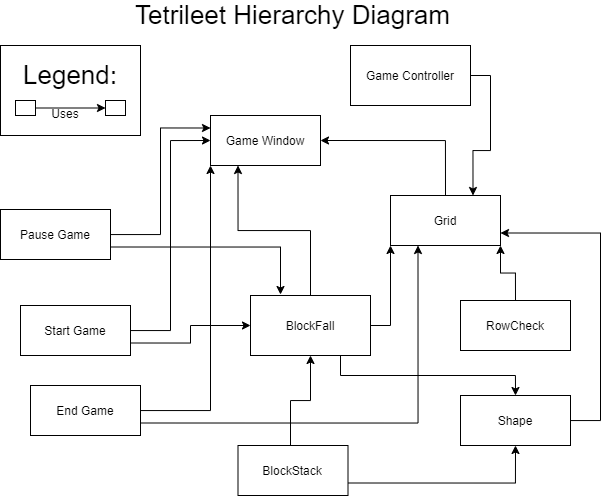
\includegraphics[width=0.7\textwidth]{Heirarchy.png}
\caption{Use hierarchy among modules}
\label{FigUH}
\end{figure}


\section{Schedule} \label{SecUse}

The Gantt chart of our project schedule is located in this repo, at\\ 3xa3-L01-group-15/ProjectSchedule/group115.gan.

\end{document}